\documentclass{article}
\usepackage[utf8]{inputenc}

\title{MI-PAA: Problém batohu, úloha 3}
\author{Josef Doležal}

\usepackage{natbib}
\usepackage[czech]{babel}
\usepackage{a4wide}
\usepackage{graphicx}
\usepackage{float}

\begin{document}

\maketitle

\section{Úvod}
Problémem batohu se nazývá úloha, ve které je za úkol pro množinu $n$ předmětů a batoh o maximální nosnosti $m$ určit, jak předměty do batohu vložit tak, aby v součtu měly co největší hodnotu a zároveň nebyla překročena maximální nosnost batohu.

Vstupem je tedy seznam $n$ předmětů (dvojic váha-cena) a maximální nosnost batohu $m$.
Výstupem je v součtu nejvyšší možná cena předmětů, jejichž váha dohromady nepřekročí nosnost.

\section{Zadání úlohy}

\begin{itemize}
    \item Prozkoumejte citlivost metod řešení problému batohu na parametry instancí generovaných generátorem náhodných instancí. Máte-li podezření na další závislosti, modifikujte zdrojový tvar generátoru.
    \item Na základě zjištění navrhněte a proveďte experimentální vyhodnocení kvality řešení a výpočetní náročnosti.
    \item Zkoumejte zejména následující metody: hrubá síla, metoda větví a hranic, dynamické programování a heuristika (poměr cena/váha).
    Pozorujte zejména závislosti výpočetního času (případně počtu testovaných stavů) a rel. chyby (v případě heuristiky) na: maximální váze věcí, maximální ceně věcí, poměru kapacity batohu k sumární váze a granularitě.
\end{itemize}

\section{Rámcový popis řešení}

Pro určení citlivosti jednotlivých řešení problému je využito generování náhodných vstupů.
U jednotlivých vstupů jsou jsou záměrně měněny parametry generování (např. granularita, počet věcí, maximální cena, \ldots).

Pro jednotlivá řešení jsem vybral parametry takové, u kterých je vysoká pravděpodobnost, že jejich změna bude mít znatelný dopad na celkovou dobu výpočtu (exaktní metody) nebo relativní chybu (heuristika).
Zvolené parametry jsou pro jednotlivé metody následující:

\begin{itemize}
    \item Dynamické programování -- maximální cena,
    \item Metoda větví a hranic:
    \begin{itemize}
        \item maximální váha,
        \item poměr kapacity k maximální váze,
    \end{itemize}

    \item Heuristika:
    \begin{itemize}
        \item maximální cena,
        \item granularita.
    \end{itemize}
\end{itemize}

Pro jednotlivé metody řešení jsem si určil jeden proměnlivý parametr.
Na zakládě tohoto parametru jsem pro každou metodu zkoumal rozsah, pro který danná metoda vypočte řešení v přijatelném čase.

Vstupy jsou generované pomocí skriptů pro příkazovou řádku.
Pro každou dvojici metoda-parametr jsem vytvořil adresářovou strukturu se vstupy.
Zkompilovaný program bylo následně možné konfigurovat cestou ke složce se vstupy a metodou řešení.

\section{Výsledky měření}

Pro zkoumání vlastností jsme vybral dvě exaktní metody (metoda větví a hranic, dynamické programování) a heuristiku (poměr cena / váha).
Měněný parametr jsem volil tak, aby reflektoval vlastnosti jednotlivých algoritmů.


Měření bylo pro zajištění přesnosti prováděno vícekrát.

\subsection{Metoda větví a hranic -- měněný parametr váha}

\subsubsection*{Konfigurace generátoru}

\begin{table}[H]
\centering
    \begin{tabular}{ |l|l| } 
        \hline
        Parametr & Hodnota \\
        \hline
        \hline
        Počet věcí & $23$ \\
        Počet instancí & $15$ \\
        Poměr kapacity batohu k sumární váze & 0.2 \\
        Maximální váha věci & $7000 \dots 15000$ \\
        Maximální cena věci & $5000$ \\
        Exponent $k$ & $1$ \\
        Poměr velikostí věcí v batohu & $0$ \\
        \hline
    \end{tabular}
\end{table}

\subsubsection*{Výsledky měření}

\begin{figure}[H]
    \centering
    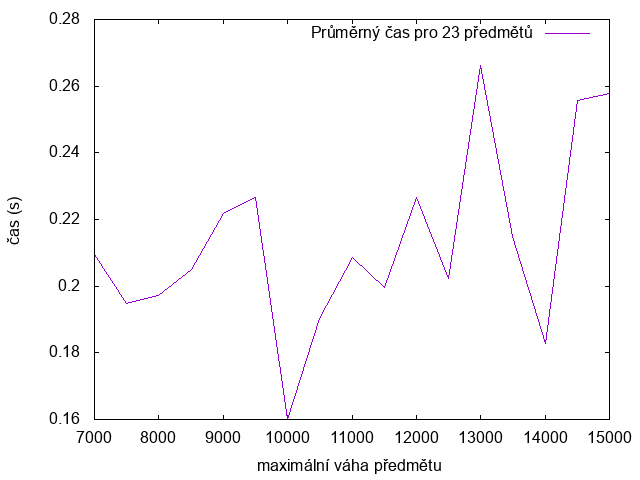
\includegraphics[width=0.8\textwidth]{inputs-bb-weight/inputs-bb-weight.png}
    \caption{Parametry k metodě větví a hranic, měněný parametr váha}
    \label{fig:g1}
\end{figure}

Z naměřených dat v grafu \ref{fig:g1} vyplývá, že metoda větví a hranic neni významně závislá na změně maximální ceny položky batohu.
To může být ovlivněno průchodem stavového prostoru, od kterého se časová složitost této metody odvíjí.
Z výsledku lze usoudit, že změna maximální ceny neovlivňuje výrazným způsobem velikost procházeného stavového prostoru.

\subsection{Metoda větví a hranic -- měněný parametr poměr kapacity batohu k sumární váze}

\subsubsection*{Konfigurace generátoru}

\begin{table}[H]
\centering
    \begin{tabular}{ |l|l| } 
        \hline
        Parametr & Hodnota \\
        \hline
        \hline
        Počet věcí & $27$ \\
        Počet instancí & $20$ \\
        Poměr kapacity batohu k sumární váze & $0.1 \dots 1.0$ \\
        Maximální váha věci & $12000$ \\
        Maximální cena věci & $100$ \\
        Exponent $k$ & $1$ \\
        Poměr velikostí věcí v batohu & $0$ \\
        \hline
    \end{tabular}
\end{table}

\subsubsection*{Výsledky měření}

\begin{figure}[H]
    \centering
    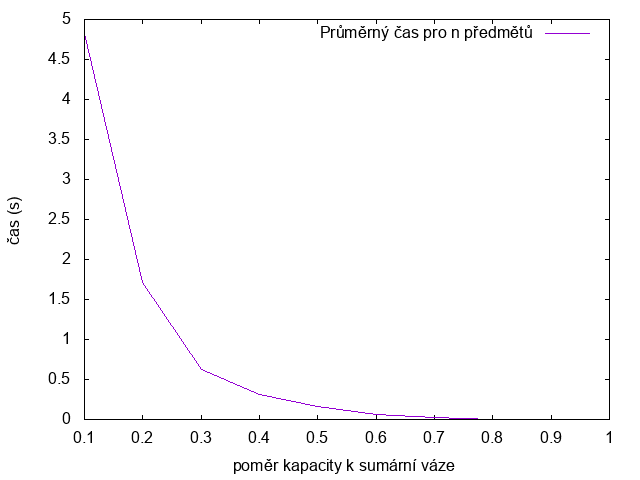
\includegraphics[width=0.8\textwidth]{inputs-bb-ratio/inputs-bb-ratio.png}
    \caption{Parametry k metodě větví a hranic, měněný parametr poměr kapacity batohu k k sumární váze}
    \label{fig:g2}
\end{figure}

Při změně poměru kapacity batohu k sumární váze je podle grafu \ref{fig:g2} vidět, že časová náročnost k nalezení optimálního řešení s rostoucím poměrem klesá.
Tento výsledek naplňuje očekávání.
S rostoucím poměrem roste pravděpodobnost, že optimální řešení nalezneme v krátkém čase a velká část statového prostoru může být při průchodu vynechána.
S roustoucím poměrem dochází k významnému zlepšení časové složitosti a algoritmus nalézá řešení ve výrazně kratším čase.

\subsection{Dynamické programování -- měněný parametr cena}

\subsubsection*{Konfigurace generátoru}

\begin{table}[H]
\centering
    \begin{tabular}{ |l|l| } 
        \hline
        Parametr & Hodnota \\
        \hline
        \hline
        Počet věcí & $27$ \\
        Počet instancí & $15$ \\
        Poměr kapacity batohu k sumární váze & $0.5$ \\
        Maximální váha věci & $200$ \\
        Maximální cena věci & $10000 \dots 20000$ \\
        Exponent $k$ & $1$ \\
        Poměr velikostí věcí v batohu & $0$ \\
        \hline
    \end{tabular}
\end{table}

\subsubsection*{Výsledky měření}

\begin{figure}[H]
    \centering
    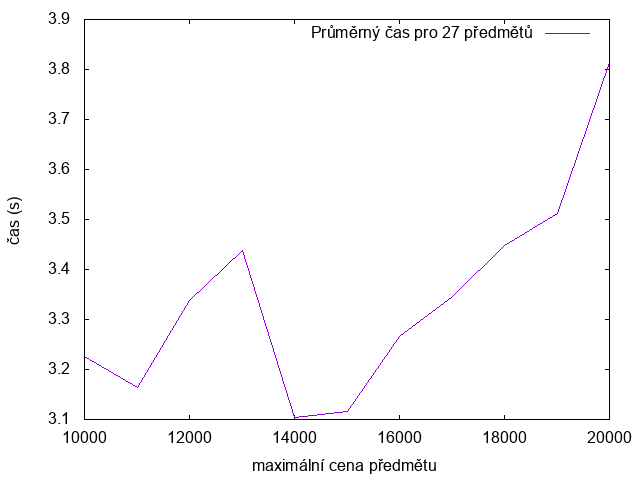
\includegraphics[width=0.8\textwidth]{inputs-dp-price/inputs-dp-price.png}
    \caption{Parametry k metodě dynamického programování, měněný parametr cena}
    \label{fig:g3}
\end{figure}

Metoda dynamického programování je dle výsledků měření uvedených v grafu \ref{fig:g3} citlivá na rostoucí cenu.
To plyne ze samotné vlastnosti tohoto pseudopolynomiálního algoritmu.
V případě řešení pomocí dekompozice podle ceny je sice algoritmus polynomiálně závislý na velikosti vstupu, ale záleží také na parametru ceny, kde je závislost až exponencionální.
Měření této metody naplnila očekávání, kde od určité počáteční hodnoty je křivka rize rostoucí.

\subsection{Parametry k heuristické metodě -- měněný parametr granularita}

\subsubsection*{Konfigurace generátoru}

\begin{table}[H]
\centering
    \begin{tabular}{ |l|l| } 
        \hline
        Parametr & Hodnota \\
        \hline
        \hline
        Počet věcí & $20$ \\
        Počet instancí & $20$ \\
        Poměr kapacity batohu k sumární váze & $0.5$ \\
        Maximální váha věci & $30$ \\
        Maximální cena věci & $100$ \\
        Exponent $k$ & $0 \dots 6$ \\
        Poměr velikostí věcí v batohu & $1$ \\
        \hline
    \end{tabular}
\end{table}

\subsubsection*{Výsledky měření}

\begin{figure}[H]
    \centering
    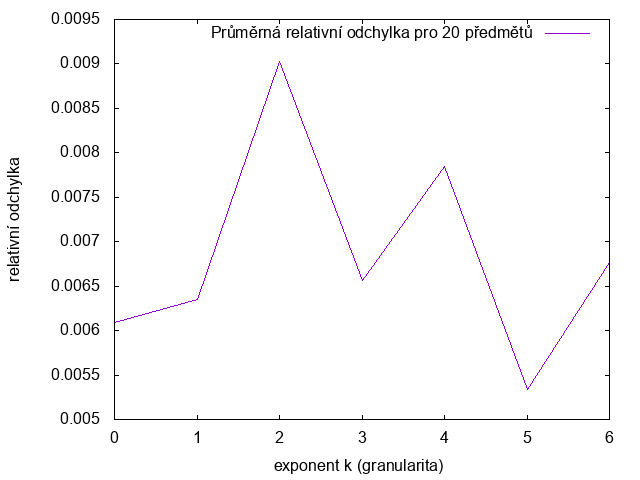
\includegraphics[width=0.8\textwidth]{inputs-heuristic-granularity/inputs-heuristic-granularity.png}
    \caption{Parametry k heuristické metodě, měněný parametr granularita}
    \label{fig:g5}
\end{figure}

Při měření kvality heuristické metody je využito měření průměrné relativní odchylky.
Z grafu \ref{fig:g4} lze usoudit, že při zvyšování granularity se odchylka od správného řešení blíží hodnotě $0.5 \%$ a má spíše klesající charakter.
Toto měření ale může být značně nepřesné z důvodu malého počtu testovacích dat (6 testovaných hodnot).
Nízký počet testovaných hodnot byl dát vysokou časovou náročností pro generování testovacích vstupů.

\subsection{Parametry k heuristické metodě -- měněný parametr cena}

\subsubsection*{Konfigurace generátoru}

\begin{table}[H]
\centering
    \begin{tabular}{ |l|l| } 
        \hline
        Parametr & Hodnota \\
        \hline
        \hline
        Počet věcí & $25$ \\
        Počet instancí & $15$ \\
        Poměr kapacity batohu k sumární váze & $0.5$ \\
        Maximální váha věci & $200$ \\
        Maximální cena věci & $10000 \dots 40000$ \\
        Exponent $k$ & $1$ \\
        Poměr velikostí věcí v batohu & $1$ \\
        \hline
    \end{tabular}
\end{table}

\subsubsection*{Výsledky měření}

\begin{figure}[H]
    \centering
    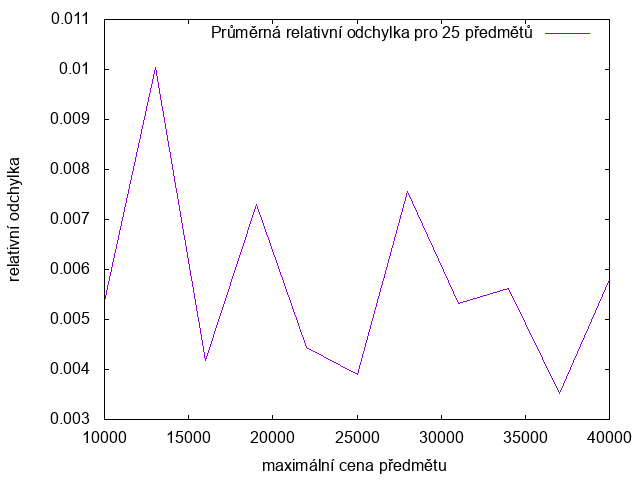
\includegraphics[width=0.8\textwidth]{inputs-heuristic-price/inputs-heuristic-price.png}
    \caption{Parametry k heuristické metodě, měněný parametr cena}
    \label{fig:g4}
\end{figure}

Obdobně jako v grafu \ref{fig:g4} tak i v grafu \ref{fig:g5} je vidět spíše klesající trend průměrné relativní odchylky.
Tato dota jsou navíc z důvodu většího počtu testovacích dat více vypovídající.
U naměřených hodnot je patrné, že žádná z hodnot nemá extrémní výkyv a lze tedy usuzovat, že kvalitu řešení cena zboží neovlivňuje nikterak drasticky.

\section{Závěr}

Naměřené údaje všech metod převážně potvrzují vlastnosti uvedené v předchozích úlohách.
Jediným výrazným překvapujícím měřením jsou vlastnosti metody větví a hranic při změně maximální váhy.
První úvahy vedou k domněnce, že s rostoucí cenou bude také růst časová složitost této metody.
Po hlubším uvážení lze ale usoudit, že velikost procházeného stavového prostoru se více odvíjí od poměru kapacity k sumární váze, což také potvrzuje druhé měření.

\end{document}
